%%% File encoding is ISO-8859-1 (also known as Latin-1)
%%% You can use special characters just like �,� and �

\chapter{Background}

\section{Problem Description}
Consider a law firm that wants to build a strong defense for its client: thousands of legal documents are available to the firm, but only a small fraction of the information contained in these documents is useful for the given case. How would lawyers go about gathering pertinent information or evidence? On one hand, the lawyers could read every word in every document available and then hope to remember it all by the end. On the other hand, such brute force is inhumanly difficult and exorbitantly expensive. More to the point, not all available information is useful. In fact, chances are that the vast majority of legal documents are irrelevant to the case at hand. For example, if the lawyers are handling a case on tax evasion, they probably do not want to read about domestic laws. The firm ultimately needs an automated and highly efficient method for organizing textual information and for retrieving the pertinent information quickly.
\\\\
This problem of organizing textual information is not new. Humans began writing somewhere around 5000 B.C. and since then have created a monolithic amount of written information. For hundreds of years, the only way to research pertinent information was to visit a library and page through book after book. The process was slow and oftentimes unfruitful. Then, with the advent of the Internet, the world rejoiced at the new availability of information and yet faced an organizational crisis. What should be done with this monolith of textual information? In what ways might all this information be useful? Most importantly, how could this information be made accessible to the general public? These questions emphasized the need for search engines, programs that could troll through large masses of web content and pick out only the relevant bits of information in real time. During the 90s, companies like Yahoo!, Ask Jeeves, and eventually Google sprang up, each offering unique methods for indexing webpages and providing speedy information retrieval \cite{SEH}. Search engines have since become a staple and keystone for day-to-day life in the twenty-first century.
\\\\
Underpinning much of search is the concept of \textbf{text mining}. Text mining refers to the organization and extraction of information from natural language documents  \cite{TextMining}. Note that search and text mining are not one and the same. Search engines typically undertake a number of steps to produce results, including indexing and query enrichment \cite{SEH}. By contrast, text mining is a more general collection of methods for extracting data from textual documents. Some examples of text mining include part-of-speech tagging, concept extraction, and sentiment analysis \cite{BYOSE:4}. In this paper, we will focus on the representation of textual documents as vectors and the categorization of textual documents into predefined categories. We will see that, with the right precautions, document categorization works out to be a fairly straightforward classification problem.
\\\\
Document categorization has many immediate applications. Lawyers may wish to automatically sort large quantities of text into semantic categories (domestic law, tax law, etc.); companies may wish to categorize incoming email and eliminate spam; search engines may want to categorize new queries to restrict their search space; and so forth \cite{BYOSE:4}. Despite its usefulness, document categorization is not trivial. It is not immediately obvious what determines whether a document belongs to a category. Language is by nature ambiguous. Some studies from cognitive science suggest that this ambiguity is evolutionarily advantageous because it eases the language learning process for young children, but that ease does not surface for computers. In particular, polysemy---the presence of multiple meanings for the same word---makes it difficult for computers to disambiguate between pairs of sentences like ``I climbed the steep \underline{bank},'' and ``I deposited a check in the \underline{bank}.'' On the other hand, language is often redundant and dilutes information with unnecessary synonyms and clarifiers like pronouns and tense. Worse yet, the categorizer may have limited access to information about the documents. In the case of web search engines, the webpages will not come with category labels; it is up to the search engine to organize the data into semantic categories.
\\\\
To address these problems, we need an effective way to encode the semantics of a document without getting lost in the ambiguity and noisy redundancy of natural language. We present methods for doing so in the proceeding section.

\section{Representation of Textual Data}
In order to extract information from documents, we must first define what we mean by document. For our purposes, a \textbf{document} is a sequence of natural language tokens  \cite{BYOSE:2}. In this sense, the sentence ``I ate an apple'' is as much a document as the entire play \textit{Hamlet}. It is worth noting that although our definition of document is limited to text, other definitions are typically more general so as to include any collection of information in written or electronic form. In fact, many of the methods for text document representation and categorization that we discuss here will apply to other types of documents as well.
\\\\
As one might expect, raw strings are not conducive to mathematical manipulation and therefore are not an ideal data representation for large-scale search. Performing string comparisons is both slow and inaccurate; the user is looking for a document semantically similar to his query, not for an exact textual match to his query. The alternative is to represent documents as vectors by defining a global list of features, and then encoding each document in terms of these features. Thus, for a corpus with $m$ features, each document will be encoded as an $m$-dimensional vector. The list of features is typically determined by the characteristics of the entire corpus. 
\\\\
Here, we will employ the term-document model. In the term-document model, each feature corresponds to a term from the collection of all terms taken over all documents \cite{BYOSE:2}. Its value is given by the number of times that term appears in the document. For example, let $d = [d_1 \ d_2 \ \dots \ d_m]^T$ be the feature vector given by some new document, and $\mathcal{V}$ the collection of all terms (features) in the corpus. If term $v \in \mathcal{V}$ appears in the document $k$ times, we have $d_v = k$, noting that we let each term correspond to some index of the vector. Unfortunately, this encoding is still meaningless: a document might contain the word ``the'' in 1256 different places, giving it a large feature value, but that does not mean the word ``the'' is semantically salient. As a first step to remedying this, we need to weight each term inversely to how often it is used throughout the corpus, under the assumption that rarer words better identify the semantics of a document. This encoding is called the \textbf{term frequency-inverse document frequency (tf-idf)} because each term frequency feature is multiplied by the inverse of its corpus frequency.
\begin{figure}[h]
  \centering
  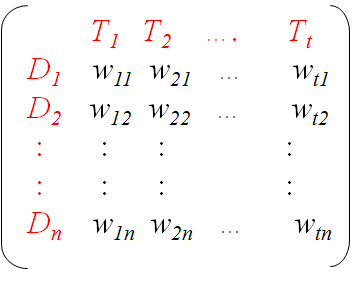
\includegraphics[width=50mm, scale=0.5]{03_Graphics/tfidf.png}
  \caption{Document matrix where rows ($D_i$) are document vectors and columns ($T_i$) are tf-idf weights, from \cite{MS:TFIDF}}
  \label{fig:docmatrix}
\end{figure}
\\
This encoding gives rise to a natural similarity measure for documents, namely, the normalized dot product or cosine similarity measure. For documents $d_i$ and $d_j$ in the same corpus, the similarity of $d_i$ and $d_j$ is given by $\frac{d_i^{\intercal}d_j}{||d_i||\cdot||d_j||}$. Any features that are not shared by both documents will be zeroed out, so the result is entirely determined by tf-idf values for terms that appear in both documents. Moreover, since common terms will have low weights, they will contribute little to the dot product, while shared rare terms like ``interpolate'' or ``Nietzsche'' will contribute a great deal to the dot product. This is in line with our assumption that rare words probably have semantic salience. Note that we can also obtain a measure of term similarity in this way: if we arrange each document vector as a row in a matrix, we see that the columns form feature vectors for terms, where the $i^{th}$ feature is the tf-idf of that term in document $i$. This is an intuitive representation because terms that are semantically similar will likely appear in the same document. As one might expect, the normalized dot product of two term vectors gives a rough similarity measure of those terms  \cite{BYOSE:3}. 
\\\\
The term-document model is good at highlighting the semantic hotspots of a document---that is, the rare and potentially salient words---but it does not completely remove the redundancy of natural language. We must take other steps to reduce the noise from each document. One cheap solution is to remove short words from the feature space. This works because most short words are either articles or acronyms that are spelled out elsewhere in the text; however, there is still the risk of eliminating important information. Supposing we chose to remove all words of length three or less, say, in an effort to remove ``the'' from consideration, we might in the process eliminate the word ``bee'' from a text on endangered species, which is clearly undesirable. A more effective approach is to remove all \textbf{stop words} from the corpus, where a stop word is defined to be any word that contributes no information to the text, like ``the.'' The collection of stop words varies from case to case.
\\\\
Finally, before featurizing a corpus, we should make sure to remove any unnecessary prefixes or suffixes from each word, so that the words ``walk'' and ``walked'' are not considered separate features. This is called \textbf{stemming} \cite{BYOSE:1}. We omit the details.

\section{Latent Semantic Analysis}

In the previous section, we hinted that an entire corpus can be represented as a single matrix, where each row is a document vector. In fact, this representation exposes information about the corpus as a whole, and provides a means for extracting and simplifying that information.
\\\\
The astute reader will have noticed that the term-document model results in sparse vectors with many dimensions. Some of these dimensions are virtually useless, while others match the semantic category of a document but are zeroed out because the term represented by that dimension does not appear in the document. Despite our efforts at normalization with the term-document model, we still have not accounted for the problem of synonomy. We want to uncover the latent semantic structures that underly a corpus. In other words, we would like to discover the semantic relationships between terms and to combine synonyms such that our term vectors (the columns of the corpus matrix) represent something closer to a semantic category than a specific word. For example, ``chihuahua'' and ``dog'' are different words but both belong to the same semantic category. From a search perspective, we would like to consider a document that mentions chihuahuas as similar to a query for dogs. 
\\\\
We can achieve this dimensionality reduction by performing \textbf{latent semantic analysis (LSA)} on the corpus matrix. Latent semantic analysis involves finding a low-rank approximation of the corpus matrix. To do this, we apply the Eckart-Young theorem, which states that the best $k$-rank approximation for an $n \times m$ matrix, $k < m$, over some unitarily invariant norm is given by the outer product of the the first $k$ singular values and vectors of the original matrix. Formally, if the singular value decomposition of a matrix $A$ is given by $\sum_{i=1}^r\sigma_iu_iv_i^{\intercal}$, then the best $k$-rank approximation to $A$ is:
	$$A_k = \sum_{i=1}^k\sigma_iu_iv_i^{\intercal}$$ 
\\\\
We can think of this approximation in a number of ways. On one hand, some dimensions (terms) are being zeroed out, namely those dimensions with the least semantic significance across all documents, so we are reducing the sway of redundant or unhelpful term features. On the other hand, terms that were previously zeroed out in certain documents may now be nonzero. We can think of this as stretching terms into $k$ of the most salient semantic categories across the entire corpus, where each term has varying membership to each category \cite{BYOSE:3}. Notice that this analysis depends heavily on the assumption that similar words in semantic space will generally co-occur in documents.
\\\\
Typically, we choose $k \approx 100$, though studies have shown that there are good results with $k$ as small as 50 or as large as 1000 \cite{BYOSE:3}. 

\section{Categorization of Textual Documents}
We now have the tools to discuss methods of document categorization. As we have suggested, document categorization boils down to a supervised classification problem with a few modifications. We will discuss and compare three different classifiers as they relate to document categorization: k-nearest neighbors (kNN), least squares (LS), and support vector machines (SVMs).

\subsection{Formalization}

We begin by formalizing document categorization as a classification problem. Let $\mathcal{D}$ denote the set of all documents in the corpus and $\mathcal{C}$ the set of all semantic categories, which we take to be predefined. Formally, our input is a set of tuples $(d_i, C_i)$, where $d_i \in \mathcal{D}$ denotes the tf-idf vector for document $i$ and $C_i \subset \mathcal{C}$ denotes the set of categories to which document $i$ belongs. Notice that the labels are not individual objects but sets. It is easy to imagine cases where a document belongs to multiple semantic categories. Thus, for a new, unlabeled document $d_*$ we would like to predict the set of semantic categories $C_*$ to which it belongs.
\\\\
Already it should be clear that this problem is more complicated than other classification problems. The classifiers we will discuss are prototypically binary classifiers---that is, new examples belong to exactly one of two classes---so we will have to find an adequate modification that (a) can classify examples into more than just two categories and (b) allows examples to belong to more than one category. This is called the problem of \textbf{multiple classification}, and we address it for each classification method in turn.

\subsection{k-Nearest Neighbors}
The first classification scheme we will discuss is \textbf{k-nearest neighbors} \cite{kNNArticle}. We can imagine our document vectors as points in $m$-dimensional semantic space, where spatial proximity correlates with semantic similarity. The kNN classification scheme grounds itself in this idea and assumes that new, unlabeled examples will be similar to the labeled examples that are nearby in feature space. Specifically, for $k > 0$, the kNN classifier chooses the $k$ points from the training data that are closest in Euclidean distance to a new data point and takes the majority class of the nearest neighbors to be the class of the new example. To visualize this, consider Figure \ref{fig:knn}: if $k = 3$, then the new point would be labeled as red since two of its three closest neighbors are red; if $k = 5$, the new point would be labeled blue.
\begin{figure}[h]
	\centering
	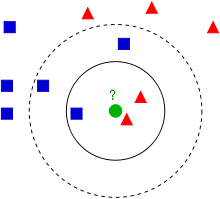
\includegraphics[width=50mm, scale=0.5]{03_Graphics/knn.png}
	\caption{Example of a k-NN classifier, from \cite{Wikipedia:kNN}. The test sample (green circle) will be classified as either the class of red triangles or blue squares.}
	\label{fig:knn}
\end{figure}
kNN has the advantage of naturally addressing the multiple-classification problem. For each of the $k$ nearest neighbors, we increment the vote count for each class to which that neighbor belongs. We then ignore classes whose vote counts are lower than some constant threshold and choose the $r$ most-voted of the remaining classes to be our classification. 
\\\\
This kNN classification scheme has been shown to work well for document categorization. In fact, it is the most common method of document categorization because it is easy to implement and because it does not require us to train a classifier \cite{BYOSE:4}. The latter advantage is also a significant disadvantage, however, because new training documents must be compared to every training document to obtain a classification, which results in $O(nm)$ classification time complexity for corpora with $n$ documents and $m$ term features. This complexity is especially bad when we consider that both $n$ and $m$ are typically quite large. Another disadvantage of kNN is that the classification results may vary as you change $k$. We could compute the optimal $k$ by trying many values of $k$ and choosing the one that minimizes classification error---this results in a Pareto curve where $k$ is graphed on the $x$-axis and classification error is graphed on the $y$-axis. Unfortunately, this computation is slow and expensive for large datasets.

\subsection{Least Squares}
Next we will discuss the \textbf{least squares} classifier. Least squares classification grounds itself in the assumption that classes are determined as a linear combination of term features. We want to learn the optimal coefficients for said linear combination. To do this, we minimize the squared loss between predicted classes and actual classes in a set of training data. Formally, given our document matrix $A$, a vector $w$ of weights, and a vector $b$ of numerical labels, the predicted labels are given by $\text{sign}(Aw)$, where the sign is taken element-wise, and we wish to find $\text{argmin}_w ||Aw - b||_2^2 = \hat{w}$. We can then classify a new document $a$ by evaluating $\text{sign}(a^\intercal \hat{w})$, where again the sign is element-wise. Practically, we can solve this problem by computing the pseudoinverse of $A$ and multiplying it by $b$.
\begin{figure}[h]
	\centering
	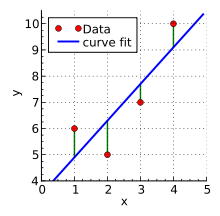
\includegraphics[width=50mm, scale=0.5]{03_Graphics/leastsquares.png}
	\caption{A plot of data points with a blue least squares best fit line, from \cite{Wikipedia:LS}.}
	\label{fig:ls}
\end{figure}
As we've already seen, least squares on its own is not sufficient for document categorization because it cannot accurately distinguish more than two categories. In practice, we have two choices for multiple-classification schemes with binary classifiers. The first scheme is called \textbf{one-vs-all classification}, where one classifier is trained per category that learns only to distinguish its category from all others, and each classifier returns a continuous measure of class membership as opposed to a strict yes/no answer. Thus, if there are $k$ classes, then the one-vs-all schema trains $k$ different classifiers. The second schema is called \textbf{one-vs-one classification}, where $k(k-1)/2$ binary classifiers are trained, one for each unique pair of categories. Each classifier learns to distinguish between its two given categories. To classify a new example, we apply each classifier and choose the class with the majority vote.
\\\\
Both schema have advantages and disadvantages. However, one-vs-one classification tends to be the method of choice. Although it requires us to train more classifiers, we train each classifier on fewer examples. Moreover, the voting system helps to eliminate noise in the data and gives us a means of determining multiple-class membership for new examples---we need only iterate through the class votes.
\\\\
If we again think of document vectors as points in semantic space, then least squares finds the optimal hyperplanes for separating each pair of categories. Of course, the data might not be linearly separable, but we can make it separable lifting each point into a higher-dimensional space with kernel methods, and then we can apply least squares in the new feature space. We can do the same with the SVM. We omit the details.
\\\\
Least squares tends to perform well on document categorization tasks, particularly when the semantic structure of a corpus has been compacted with latent semantic analysis \cite{BYOSE:2}. Although the kernelized SVM is preferred to least squares in most applications, the two classification schemes have comparable performance. In both cases, the loss function is generally regularized with respect to the $L_2$ norm so as to ensure that no one term carries too much weight. This makes sense because the semantics of a document are almost never determined by a single term---rather, the semantics depend on the culmination of all terms and concepts presented in the document.

\subsection{Support Vector Machines}
The last classifier we will mention is the \textbf{support vector machine}. Formally, the support vector machine learns the optimal weight vector $w$ such that the hinge loss given by $\sum_{i=0}^n(1 - y_ia_i^{\intercal}w)_+$ is minimized, where $y_i$ is the label of the $i^{th}$ document, $a_i$ is the feature vector for the $i^{th}$ document, and the last subscript represents a soft threshold.
\\\\
Like least squares, the SVM finds a separating hyperplane between two classes. However, least squares struggles with outliers in the data. If a point is classified ``too correctly,'' that is, it is classified correctly but is far from the decision boundary, then its squared distance from the hyperplane will be large and thus the least squares hyperplane will be pulled toward that data point. By contrast, the SVM does not penalize data that are classified very well. This is because the SVM finds the hyperplane with the greatest margin between the two classes, as shown in Figure \ref{fig:ls}. The resulting hyperplane depends only on the points closest to it.
\begin{figure}[h]
	\centering
	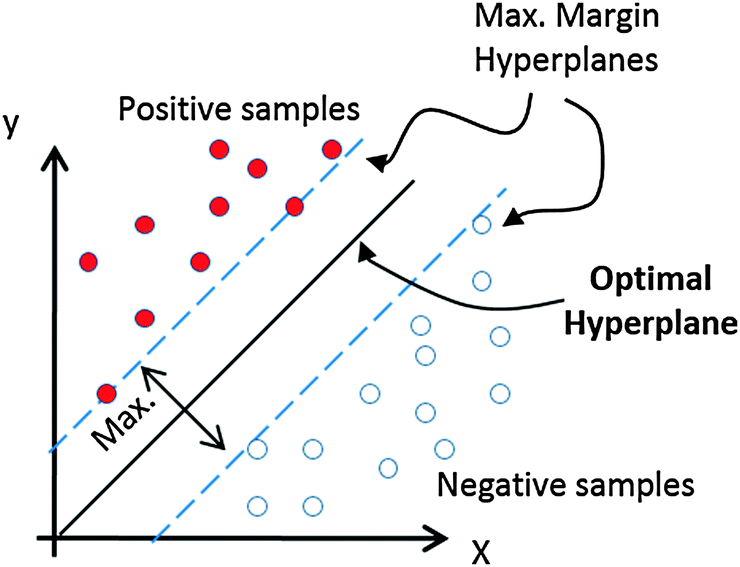
\includegraphics[width=70mm, scale=0.5]{03_Graphics/svm.png}
	\caption{A SVM hyperplane separating two classifications with a maximum margin, from \cite{RSC:SVM}.}
	\label{fig:ls}
\end{figure}
As we have suggested, the SVM implemented with a one-vs-one multiple classification schema is the preferred classifier for document categorization. One reason for this is that we expect documents to be linearly separable in semantic space, and SVMs are known to learn robust linear separators. In fact, studies and experiments with the Reuters-21578 corpus (for which we will be constructing a search engine) show that almost every semantic category in the corpus is linearly separable by using an SVM, as demonstrated in \cite{BYOSE:2} and \cite{BYOSE:4}. Additionally, SVMs lend themselves to high-dimensional feature spaces like textual corpora because they are built to combat overfitting. This is a result of the large margins enforced by SVMs---we can think of SVMs as leaving a lot of room for new examples. 
\\\\
SVMs perform even more favorably in conjunction with Tikhonov regularization \cite{BYOSE:2}. After we perform LSA, we expect few features to be irrelevant. Most or all of the remaining term features should contribute to the meaning of the document. As such, we want to avoid regularizers like the $L_1$ norm that promote sparse solutions. We also should not regularize with a quantizing regularizer like the $L_\infty$ norm because we do expect some terms to be more important than others in determining a document's semantics.
\\\\
The last advantage for SVMs we will mention is their practical  